\chapter{Cascading Power Failures}

A cascading failure is a process in which the failure of a set of components weakens the system and increases the likelihood of future failures of components.  The application to power systems has seen interest due to the large cost to society when one does occur.  It has recently been studied in multiple papers, including a series where Dobson et. al. develop their OPA model.  This models the interaction between the short term force of blackouts and the long term effects of growth and economics for developing the power system.  \\

In 2001, Dobson et. al. argued that the power system has self-organized into a dynamic equillabrium where blackouts of all sizes occur \cite{Dobson_2001}.  Their following paper furthers their case for this model representing behavior from the North American power systems.  They note that the average frequency of blackouts in the United states is 13 days and has been the same for 30 years \cite{Carreras_2004}, which appears to represent an equillibrium.  The distribution of blackouts from North American Electrical Reliability Council (NERC) data for the last 15 years follows a power tail curve with an exponent of around $-1.3\pm.2$ \cite{Carreras_2004}.  The model approximates the interaction between the physical system, economic, regulatory, and political responses and blackouts.  The results were consistent with available North American data \cite{Carreras_2004}. \\

This work will develop a planning model that will incorporate the effects of cascading power failures.  The end-use of this model will be developing transmission capacity effectively and designing operating standards for power systems.  It will use the OPA model to examine the effects of cascading power failures in power systems under a set of contingencies.  Two different approaches will be used, a simulation-based optimization algorithm and a multi-stage stochastic program.  \\

The simulation-based approach will directly use OPA model and will solve the problem in a timely manner.  The OPA model will be devleloped in respect to the variables of design, demand, contingencies, and the random process of cascading.  It is a flow based model which approximates the power flow of a topological network with known power injects at the nodes using the DC power flow model.  Hard capacity constraints are used and lines at maximum capacity are outaged with a given probability.  This process repeats based on the new topology until the system becomes stable (no outages). Since the output of this simulation is random, statistics will be used to estimate the confidence of the output.  By varying demand and continencies, the model will find a good design which is robust to cascading power failures.  \\

The multi-stage stochastic program will approximate the OPA model with a mixed-integer program that models the stages of the cascading process.  Since tochastic programs are known to be computationally intensive with even a modest size in a limited number of stages, this approach will be less scalable to large grid.  By using probablistic models of cascading failures, \cite{Dobson_2005} it may be possible to reduce this to a two-stage stochastic program.  The first stage of the model will be design.  Variables for capacity expansion or operating standards will be resolved before any knowledge of the cascading process is known.  This resulting power system will then be hit with multiple contingencies, in which load shed and particularly cascading failures may occur.  The resulting loss of load will be penalized based on the stage of the cascade.  The objective of this program will be to optimize the design variables within a give budget that minimizes the weighted load shed.  

TRANSITION PARAGRAPH TO UNDERSTANDING REAL WORLD EXAMPLE TO DRIVE MODELING EFFORTS


\section{Northeast Blackout, 2003}

Need to show example of what trying to model

\subsection{Chain of Events}

timeline of events through cascade period

\subsection{Costs of Cascade}

what were damages done


%\documentclass{standalone}
%\begin{document}

\def \sc     { .65 }
\def \lw     { 1.25pt }

\begin{figure}
\centering
\begin{subfigure}[b]{.46\linewidth}
\begin{tikzpicture}[line width=\lw,scale=\sc]

\node[circle,fill=blue!20] (one) at (3,0) {\small 1};
\node[circle,fill=red!20] (two) at (5,0) {\small 2};
\node[rectangle,fill=green!20] (three) at (7,1) {\small 3};
\node[rectangle,fill=green!20] (four) at (5,1.75) {\small 4};
\node[rectangle,fill=green!20] (five) at (3,1.75) {\small 5};
\node[circle,fill=red!20] (six) at (2,3) {\small 6};
\node[rectangle,fill=green!20] (seven) at (5,3) {\small 7};
\node[circle,fill=red!20] (eight) at (3.85,3.45) {\small 8};
\node[rectangle,fill=green!20] (nine) at (7,3) {\small 9};
\node[rectangle,fill=green!20] (ten) at (5.85,4.1) {\small 10};
\node[rectangle,fill=green!20] (eleven) at (3.75,5) {\small 11};
\node[rectangle,fill=green!20] (twelve) at (2.35,5) {\small 12};
\node[rectangle,fill=green!20] (thirteen) at (.81,4.2) {\small 13};
\node[rectangle,fill=green!20] (fourteen) at (4,6) {\small 14};


\draw (one) -- (two) ;
\draw (one) -- (five);
\draw (two) -- (three) ; 
\draw (two) -- (four) ; 
\draw (two) -- (five) ; 
\draw (three) -- (four) ; 
\draw[red] (four) -- (five) ; 
\draw (four) -- (seven);
\draw (four) -- (nine);
\draw (five) -- (six) ; 
\draw (six) -- (eleven) ; 
\draw (six) -- (twelve) ; 
\draw (six) -- (thirteen) ; 
\draw (seven) -- (eight) ; 
\draw (seven) -- (nine) ; 
\draw (nine) -- (ten) ; 
\draw (nine) .. controls +(up:1.2cm) .. (fourteen) ;
\draw[red] (ten) -- (eleven); 
%\draw[red] (eleven) -- (twelve); 
\draw[red] (twelve) -- (thirteen);
\draw (thirteen) .. controls +(up:1.2cm) .. (fourteen) ; 
\end{tikzpicture}
\caption{Initial Event: The three red lines are outaged and the power flow redistributes.}
\end{subfigure}
\begin{subfigure}[b]{.46\linewidth}
\begin{tikzpicture}[line width=\lw,scale=\sc]

\node[circle,fill=blue!20] (one) at (3,0) {\small 1};
\node[circle,fill=red!20] (two) at (5,0) {\small 2};
\node[rectangle,fill=green!20] (three) at (7,1) {\small 3};
\node[rectangle,fill=green!20] (four) at (5,1.75) {\small 4};
\node[rectangle,fill=green!20] (five) at (3,1.75) {\small 5};
\node[circle,fill=red!20] (six) at (2,3) {\small 6};
\node[rectangle,fill=green!20] (seven) at (5,3) {\small 7};
\node[circle,fill=red!20] (eight) at (3.85,3.45) {\small 8};
\node[rectangle,fill=green!20] (nine) at (7,3) {\small 9};
\node[rectangle,fill=green!20] (ten) at (5.85,4.1) {\small 10};
\node[rectangle,fill=green!20] (eleven) at (3.75,5) {\small 11};
\node[rectangle,fill=green!20] (twelve) at (2.35,5) {\small 12};
\node[rectangle,fill=green!20] (thirteen) at (.81,4.2) {\small 13};
\node[rectangle,fill=green!20] (fourteen) at (4,6) {\small 14};

\draw[red] (one) -- (two) ;
\draw (one) -- (five);
\draw (two) -- (three) ; 
\draw[red] (two) -- (four) ; 
\draw (two) -- (five) ; 
\draw[red] (three) -- (four) ; 
%\draw (four) -- (five) ; 
\draw (four) -- (seven);
\draw (four) -- (nine);
\draw (five) -- (six) ; 
\draw (six) -- (eleven) ; 
\draw (six) -- (twelve) ; 
\draw (six) -- (thirteen) ; 
\draw (seven) -- (eight) ; 
\draw (seven) -- (nine) ; 
\draw (nine) -- (ten) ; 
\draw (nine) .. controls +(up:1.2cm) .. (fourteen) ;
%\draw (ten) -- (eleven); 
%\draw (twelve) -- (thirteen);
\draw (thirteen) .. controls +(up:1.2cm) .. (fourteen) ; 
\end{tikzpicture}
\caption{Stage 1: Lines 1-2, 2-4, and 3-4 are overloaded. Lines 1-2 and 3-4 fail, but line 2-4 remains in operation at an overloaded state. }

\end{subfigure}
\begin{subfigure}[b]{.46\linewidth}

\begin{tikzpicture}[line width=\lw,scale=\sc]

\node[circle,fill=blue!20] (one) at (3,0) {\small 1};
\node[circle,fill=red!20] (two) at (5,0) {\small 2};
\node[rectangle,fill=green!20] (three) at (7,1) {\small 3};
\node[rectangle,fill=green!20] (four) at (5,1.75) {\small 4};
\node[rectangle,fill=green!20] (five) at (3,1.75) {\small 5};
\node[circle,fill=red!20] (six) at (2,3) {\small 6};
\node[rectangle,fill=green!20] (seven) at (5,3) {\small 7};
\node[circle,fill=red!20] (eight) at (3.85,3.45) {\small 8};
\node[rectangle,fill=green!20] (nine) at (7,3) {\small 9};
\node[rectangle,fill=green!20] (ten) at (5.85,4.1) {\small 10};
\node[rectangle,fill=green!20] (eleven) at (3.75,5) {\small 11};
\node[rectangle,fill=green!20] (twelve) at (2.35,5) {\small 12};
\node[rectangle,fill=green!20] (thirteen) at (.81,4.2) {\small 13};
\node[rectangle,fill=green!20] (fourteen) at (4,6) {\small 14};

%\draw[red] (one) -- (two) ;
\draw (one) -- (five);
\draw (two) -- (three) ; 
\draw[red] (two) -- (four) ; 
\draw[red] (two) -- (five) ; 
%\draw[red] (three) -- (four) ; 
%\draw (four) -- (five) ; 
\draw (four) -- (seven);
\draw (four) -- (nine);
\draw (five) -- (six) ; 
\draw (six) -- (eleven) ; 
\draw (six) -- (twelve) ; 
\draw[red] (six) -- (thirteen) ; 
\draw (seven) -- (eight) ; 
\draw[red] (seven) -- (nine) ; 
\draw (nine) -- (ten) ; 
\draw (nine) .. controls +(up:1.2cm) .. (fourteen) ;
%\draw (ten) -- (eleven); 
%\draw (twelve) -- (thirteen);
\draw (thirteen) .. controls +(up:1.2cm) .. (fourteen) ; 
\end{tikzpicture}
\caption{Stage 2: On the new topology, lines 2-5, 6-13, and 7-9 become overloaded.  The cascade progresses by outaging lines 2-4 and 7-9.}
\end{subfigure}
\begin{subfigure}[b]{.46\linewidth}
\begin{tikzpicture}[line width=\lw,scale=\sc]


\node[circle,fill=blue!20] (one) at (3,0) {\small 1};
\node[circle,fill=red!20] (two) at (5,0) {\small 2};
\node[rectangle,fill=green!20] (three) at (7,1) {\small 3};
\node[rectangle,fill=green!20] (four) at (5,1.75) {\small 4};
\node[rectangle,fill=green!20] (five) at (3,1.75) {\small 5};
\node[circle,fill=red!20] (six) at (2,3) {\small 6};
\node[rectangle,fill=green!20] (seven) at (5,3) {\small 7};
\node[circle,fill=red!20] (eight) at (3.85,3.45) {\small 8};
\node[rectangle,fill=green!20] (nine) at (7,3) {\small 9};
\node[rectangle,fill=green!20] (ten) at (5.85,4.1) {\small 10};
\node[rectangle,fill=green!20] (eleven) at (3.75,5) {\small 11};
\node[rectangle,fill=green!20] (twelve) at (2.35,5) {\small 12};
\node[rectangle,fill=green!20] (thirteen) at (.81,4.2) {\small 13};
\node[rectangle,fill=green!20] (fourteen) at (4,6) {\small 14};

%\draw[red] (one) -- (two) ;
\draw (one) -- (five);
\draw (two) -- (three) ; 
%\draw[red] (two) -- (four) ; 
\draw[red] (two) -- (five) ; 
%\draw[red] (three) -- (four) ; 
%\draw (four) -- (five) ; 
\draw[red] (four) -- (seven);
\draw[red] (four) -- (nine);
\draw (five) -- (six) ; 
\draw (six) -- (eleven) ; 
\draw (six) -- (twelve) ; 
\draw[red] (six) -- (thirteen) ; 
\draw (seven) -- (eight) ; 
%\draw[red] (seven) -- (nine) ; 
\draw (nine) -- (ten) ; 
\draw (nine) .. controls +(up:1.2cm) .. (fourteen) ;
%\draw (ten) -- (eleven); 
%\draw (twelve) -- (thirteen);
\draw[red] (thirteen) .. controls +(up:1.2cm) .. (fourteen) ; 
\end{tikzpicture}
\caption{Stage 3: This has the effect of routing all power destined for load 8 through the north passage. Lines 13-14, 4-7, and 4-9 are outaged along the path. }
\end{subfigure}

\begin{subfigure}[b]{.46\linewidth}
\begin{tikzpicture}[line width=\lw,scale=\sc]


\node[circle,fill=blue!20] (one) at (3,0) {\small 1};
\node[circle,fill=red!20] (two) at (5,0) {\small 2};
\node[rectangle,fill=green!20] (three) at (7,1) {\small 3};
\node[rectangle,fill=green!20] (four) at (5,1.75) {\small 4};
\node[rectangle,fill=green!20] (five) at (3,1.75) {\small 5};
\node[circle,fill=red!20] (six) at (2,3) {\small 6};
\node[rectangle,fill=green!20] (seven) at (5,3) {\small 7};
\node[circle,fill=red!20] (eight) at (3.85,3.45) {\small 8};
\node[rectangle,fill=green!20] (nine) at (7,3) {\small 9};
\node[rectangle,fill=green!20] (ten) at (5.85,4.1) {\small 10};
\node[rectangle,fill=green!20] (eleven) at (3.75,5) {\small 11};
\node[rectangle,fill=green!20] (twelve) at (2.35,5) {\small 12};
\node[rectangle,fill=green!20] (thirteen) at (.81,4.2) {\small 13};
\node[rectangle,fill=green!20] (fourteen) at (4,6) {\small 14};


%\draw[red] (one) -- (two) ;
\draw (one) -- (five);
\draw (two) -- (three) ; 
%\draw[red] (two) -- (four) ; 
\draw[red] (two) -- (five) ; 
%\draw[red] (three) -- (four) ; 
%\draw (four) -- (five) ; 
%\draw (four) -- (seven);
%\draw (four) -- (nine);
\draw (five) -- (six) ; 
\draw (six) -- (eleven) ; 
\draw (six) -- (twelve) ; 
\draw (six) -- (thirteen) ; 
\draw (seven) -- (eight) ; 
%\draw[red] (seven) -- (nine) ; 
\draw (nine) -- (ten) ; 
\draw (nine) .. controls +(up:1.2cm) .. (fourteen) ;
%\draw (ten) -- (eleven); 
%\draw (twelve) -- (thirteen);
%\draw (thirteen) .. controls +(up:1.2cm) .. (fourteen) ; 
\end{tikzpicture}
\caption{Stage 4:  Finally, line 2-5 that is still overloaded is outaged. }
\end{subfigure}
\begin{subfigure}[b]{.46\linewidth}
\begin{tikzpicture}[line width=\lw,scale=\sc]


\node[circle,fill=blue!20] (one) at (3,0) {\small 1};
\node[circle,fill=red!20] (two) at (5,0) {\small 2};
\node[rectangle,fill=green!20] (three) at (7,1) {\small 3};
\node[rectangle,fill=green!20] (four) at (5,1.75) {\small 4};
\node[rectangle,fill=green!20] (five) at (3,1.75) {\small 5};
\node[circle,fill=red!20] (six) at (2,3) {\small 6};
\node[rectangle,fill=green!20] (seven) at (5,3) {\small 7};
\node[circle,fill=red!20] (eight) at (3.85,3.45) {\small 8};
\node[rectangle,fill=green!20] (nine) at (7,3) {\small 9};
\node[rectangle,fill=green!20] (ten) at (5.85,4.1) {\small 10};
\node[rectangle,fill=green!20] (eleven) at (3.75,5) {\small 11};
\node[rectangle,fill=green!20] (twelve) at (2.35,5) {\small 12};
\node[rectangle,fill=green!20] (thirteen) at (.81,4.2) {\small 13};
\node[rectangle,fill=green!20] (fourteen) at (4,6) {\small 14};


%\draw[red] (one) -- (two) ;
\draw (one) -- (five);
\draw (two) -- (three) ; 
%\draw (two) -- (four) ; 
%\draw[red] (two) -- (five) ; 
%\draw[red] (three) -- (four) ; 
%\draw (four) -- (five) ; 
%\draw (four) -- (seven);
%\draw (four) -- (nine);
\draw (five) -- (six) ; 
\draw (six) -- (eleven) ; 
\draw (six) -- (twelve) ; 
\draw (six) -- (thirteen) ; 
\draw (seven) -- (eight) ; 
%\draw[red] (seven) -- (nine) ; 
\draw (nine) -- (ten) ; 
\draw (nine) .. controls +(up:1.2cm) .. (fourteen) ;
%\draw (ten) -- (eleven); 
%\draw (twelve) -- (thirteen);
%\draw (thirteen) .. controls +(up:1.2cm) .. (fourteen) ; 
\end{tikzpicture}
\caption{Stage 5:  The system stabilizes into islands with generator 1 serving load 6.  However, loads 2 and 8 are out of service.}
\end{subfigure}
\caption{ \label{fig:cascade-example} \small An example of a cascading power failure. Node 1 is a generator and nodes 2, 6, and 8 are loads.}
\end{figure}

%\end{document}


\section{OPA Model math}

Now the notation developed for power grid analysis will be used to describe the short term, OPA model.  This part of the model describes how the power system responds to an initial exogenous event with respect to the cascading process.  The process starts with an operating grid being hit by an exogenous event.  This event causes the initial set of line failures.  The DC power flow model will be solved with the new grid constraints in order to find the resulting power flows.  Now, if any of the power flows are at their line capacity, they will fail with a given probability.  This may create a set of line outages, which will affect the grid constraints and the process will repeat.  The cascade ends when the set of line outages is empty. \\

Let $\xi \in \Xi$ be an initial set of outages, $g_0$ the initial grid constraints, $d_0$ the nominal demand vector,  and $p$ be the probability of line outage given the line is at max capacity.  Using the OPA algorithm \ref{opa_alg}, one realization of load shed, $l_\omega$, will be calculated for the given parameters.  Since this is a random process, let $\Omega$ be the set of possible realizations from the OPA model.  In our case, the paths through the process are decided by using a realization from uniform, i.i.d, random numbers.  These numbers represent whether the line will fail or not, given it is loaded at max capacity.  So, $\Omega \subset [0,1]^{ \left| \cE \right| * T } $, where T is the number of stages for a given cascade.  

\subsection{Decision Dependent Uncertainty}
A particular realization of $\omega$ will determine the effects on the resulting grid topology and constraints for a set of outages, $\cO$.
\begin{align}
\cGR : \R^{ \magG \magE \magomega  }   \rightarrow  \R^{ \magG }  \\
	g ' = \cGR ( g , f , \omega  )
\end{align}
This determine the progression of load served through a set of stages, $\cT$ in a cascade.  Since there are a finite number of branchs, $\magT$ is bounded.  Let $\rho( t ) \equiv $ predecessor stage, then the initialization follows
\begin{align}
	g_0, \xi, d_{nom}, p \\
	( f_0, d_0 ) = \cDC ( g_0, d_{dom} ) 	\\
	g_1 \leftarrow \xi \circ g_0
\end{align}
where the last equation is the effects of the initial outages on the grid constraint set.

EFFECTIVE CAPACITY GOES HERE

\subsection{Cascade Dynamics}
Let $t$ be a stage in the cascade, the following is true for all stages in the cascade. 
\begin{align}
	( f_t , d_t ) = \cDC ( g_{ \rho (t) } , d_{ \rho (t) } )		\\
	g_t \leftarrow \cGR ( g_{ \rho (t) } , f_t , \omega_t )	
\end{align}
When the cascade stabilizes, $ g_t = g_{ \rho (t) } $, the cascade process is finished and let $t^* \leftarrow t$.\\


\subsection{Load Shed}
Finally, the load shed from the particular realization of OPA can be found.
\begin{equation}
	l = d_0  -  d_{ t^* }
\end{equation}



Let OPA represent an operator which moves from a set of initial parameters of grid constraints, initial event, demand projection, and path through state space to a real value which represents load shed through the cascading process.  That is,
\begin{align}
OPA : \R^{ \magG  \magE  \magV  \magomega }  \rightarrow  \R \\
l = OPA ( g, \xi, d, \omega )
\end{align}

\subsection{Capacity Expansion}
Capacity expansion affects the grid constraints by allowing the following
\begin{equation}\label{capexp}
	u^i = u + x
\end{equation}
Where $x$ is a vector representing additions in unit capacity to a given branch.  $x$ can be further constrained to allow for conditions such as allowing a finite number of branch changes.  

%Let $ y \in {0,1}^{ \R^{ \left| \cE  \right| } } $  
%\begin{equation}
%	\begin{align}
		

%	\end{align}
%\end{equation}

\subsection{Operating Reserves}
The power injects at generators are constrained temporally based on the distribution of operating reserves.  For $p_n$ power injects and $r_{n}$ reserves
\begin{equation}
	p_{n} \leq p_{ \rho (n) } + r_{ \rho (n) }
\end{equation}
For a given reserve margin $\gamma \in [0,1]$
\begin{equation}
	\magr\leq \gamma \magp
\end{equation}

\subsection{Redispatch}
It can also be useful to measure and control the amount of redispatch possible between stages in the cascade process.
\begin{equation}
	\delta_n = p_n - p_{ \rho (n) }
\end{equation}
RAMPING CONSTRAINTS GO HERE


\subsection{Objective}
Let the following be the load shed function.
\begin{equation}
  l = L(x, \xi, \cD, \omega )
\end{equation}
with $l \in \R^{\magV} $ being the load shed, $x$ the design variable, $\xi$ an initial outage, $\cD$ a nominal demand, and $\omega$ a path through the sample space.

An important question to answer from a modeling perspective is what is
a relevant statistic to try to optimize.  One suggestion from Ian
Dobson was to 
\[ \min_{x \in X} \Prob_{D,\xi,\omega} [L(x,\xi,D,\omega) \geq
  \tau], \]
where $\tau$ is something like 5\% of the total demand.

Another simple idea is to minimize the expected value, as is common in
stochastic programming:
\[ \min_{x \in X} \Expect_{D,\xi,\omega} [L(x,\xi,D,\omega)]. \]

Perhaps the best measure is the robust measure
\[ \min_{x \in X} \Prob_{D,\omega} \left[ \max_{\xi \in \Xi}
  L(x,\xi,D,\omega) \geq \tau \right], \]
where $\Xi$ is a set of all possible bad ``contingencies'' that the
policy-maker wishes to include.  If $|\Xi|$ is of moderate size,
evaluating 
\[ W(x,D,\omega) \defeq \max_{\xi \in \Xi} L(x,\xi,D,\omega) \]
may be done by enumeration.
In fact, if $|\Xi|$ is small, many interesting statistics could be
computed.  For example:
\[ \min_{x \in X} \Prob_{D, \omega} \left[ \cvar_{\xi,0.95}
  (L(x,\xi,D,\omega) \geq \tau) \right], \]
where $\cvar_{\xi,0.95} (F(x,\xi,D,\omega)$ is the weighted average of
the $5\%$ of the worst cases.


\section{Multi-Stage Stochastic Program}

In order to formulate this as a Stochastic Program, a mixed-integer program is needed to describe the cascading process.  It will aproximate the full OPA model, and in the limit equal.  \\

\subsection{Mixed-Integer Program}
Assume the cascade will occur in a finite number of stage, and tet $\cN$ be the set  of stages for a cascade.  The predecessor of stage $n \in \cN$ is $\rho (n)$.  The operator will have limited control over the changes it can make to the grid constraints.  This decision-dependent uncertainty complicates the modeling effort.  In this model, binary variables $z$, are used to indicate line availability.
\begin{equation} 
\left| f_n \right| \leq u z_n 
\end{equation}
where $\leq$ is component wise for each $e \in \cE$.  

When a line burns out, the phase angles and the adjoing verticies no longer are linked.  A big M constraint is introduced to account for this feature.
\begin{equation}
\left| \theta_{i,n} - \theta_{j,n} + s_e f_{e,n}  \right| \leq M ( 1 - z_{e,n} ) 
\end{equation}
where $(i,j)=e \in \cE$ and $\theta_{i,n}$ is the phase angle for $i \in \cV, n \in \cN$.  The big M is designed to enforce a logic condition while reducing the size of the relaxation.  In this case, $M = 2*\overline{\theta} + s u_n$.s

Once a line burns out, it is no longer available for the child stages.
\begin{equation}
z_n \leq z_{ \rho (n) } 
\end{equation}

Also, once load has been shed, it is no longer avaiable at child nodes. 
\begin{equation}
d_{ \rho } (n) \leq d_n
\end{equation}

In this model, lines at each stage have an {\em effective capacity} $r ( \omega )$, which is the capacity at which the line will fail under outcome $\omega$.
\begin{equation}    
	\left| f_{\rho (n)} - r ( \omega_n ) \right| \leq M ( 1 - z_n )
\end{equation}

In general, the vectors $(\theta(\omega_2), \ldots \theta(\omega_t))$
are $|E|$-dimensional random vectors that form a stochastic process.
(Sample space is $\Omega = \Omega_2 \times \Omega_3 \times \ldots
\times \Omega_T$).  We suspect that a reasonable assumption is
stagewise indepdence of the random variables $\omega_t$.  Perhaps also
reasonable is independence of $\theta_e(\omega_e) \forall e \in E$.

The stochastic program we present .  It {\em does} have knowledge of
all of the outcomes, the decision made at node $n$ {\em must be the
  same} -- must be obeyed for all child nodes.

\subsection{Multiple Contingencies}
Expand model to multiple contingencies

\subsection{Objectives}
Use weighted sum of load shed, weighting dependant on stage in cascade.



\section{Markov Decision Process}
Stages $\cT = \left\{    1, 2, \ldots, T
		\right\}	$			\\
State Space $\cS = \left\{	0 , 1   
			\right\}^{ \magE }$	\\
Action Space $\cA = \left\{     \mbox{ Discrete set of possible power flows }
			\right\}		$			\\
Probability transition matrix, describes failure of branches based on state and choosen power flow \\
Reward for chosing a particular power flow 
\subsection{Hidden Failures}
A partially observable markov decision process would work very well here for an extension. \\
belief space on availability of components	\\
$( S, A, P, R, \theta, \Omega)$, a Partially Observable Markov Decision Process (POMDP) \\
S - State space \\
A - Action Space \\
P - Transition matrix \\
R - Observation space, $ R_{j \theta}^a $, prob observe $\theta$ in state $i$, chosing action $a$ \\
$\theta$ - Observations to make		\\
$\Omega$ - Reward function		



\section{Simulation Based Analysis}
	This section will develop the statistical tools to understand the output of this random process.  The mean load shed, $\hat l $, and the $\alpha$ value at risk, $l_\alpha$, will be calculated based on a set of trials.  In order to find the confidence in the metric, sets of the metrics from many experiments will be used.

\subsection{Load Shed}

	Let $\cL$ be a set of output from the OPA algorithm \ref{opa_alg}. The the load shed of the experiment is  
\begin{equation}
	\hat l = \frac{\sum_{i \in \cL} l_i }{ \magL }   
\end{equation}

	The $\alpha$ value at risk is also a useful quantity to measure.  This value represents the $(1-\alpha)$ percentile of trials in a given experiment.  Since blackouts occur with a power law distribution, it will be important to calculate the value of the rare events.
\begin{equation}
	VaR_{\alpha}(\cL) = \mbox{max} \left\{  l \in \R : \sum_i 1_{l_i \leq l } \leq ( 1 - \alpha ) \magL \right\}  
\end{equation}

	The conditional value at risk is the weighted sum of all trials with a load shed equal to or greater than the $VaR_{\alpha}$.
\begin{equation}
		CVaR_{alpha}(\cL) = \sum_{ l \in \cL : l \geq VaR_{\alpha}(\cL)} l
\end{equation}


\subsection{Sample Variance}

For two sets of metrics, a refrence experiment, $\cM_0$, and a designed system experiment, $\cM$.
\begin{equation}
	\hat m = \frac{\sum_{m \in \cM, m_0 \in \cM_0} ( m - m_0 )}{ \magM }
\end{equation}

The standard deviation can then be calculated and an $alpha \%$ confidence interval can be found.
\begin{equation}
 StDv( \cM ) = \sqrt{ \frac{\sum  \left( m - m_0 - \hat{m} \right)^2 }{  \left( \magM-1 \right)  }} 
\end{equation}

With the following bounds, $ \underline{ \hat{m} } = \hat{m} - t_{\alpha,\magM-1} \frac{S}{\sqrt{\magM}} $, 
			$ \overline{ \hat{m} } = \hat{m} + t_{\alpha,\magM-1} \frac{S}{\sqrt{\magM}} $ \newline
The following statement holds true.
\begin{equation}
 P (  \underline{ \hat{m} } \leq m \leq  \overline{ \hat{m} } ) \geq (1-\alpha) 
\end{equation}


\subsection{Common Random Number}\label{crn}
 To ensure that $\omega$ is calculated under similiar experimental conditions, we employ a common random number approach.  For each trial $t$, every branch $k$ has a seed for a stream of random numbers.  In round $r$, the $r$th random number in the $k$th random number stream should be used.\\
 \begin{algorithmic}
 \FOR{ $k \in \mathbb{K} $}
 		\IF{ $f_k = F_k \mbox{ or } f_k = -F_k $}
 					\STATE Random Number Seed $ \gets RNS_{t,k} $
 					\FOR{ $temp \in 1,2, ..., r -1 $}
 							\STATE Generate Random Number
 					\ENDFOR
 					\STATE $p \gets U \left[ 0, 1\right] $
 					\STATE ${k} \mbox{ added to outage if } Fail(p) = 1 $
 		\ENDIF
 \ENDFOR
 \end{algorithmic}


It seems as if regardless of our approach, it may be very useful to
read and understand the seminal works by Calafirori and Campi and
Luedtke on the topic of SAA for chance constraints.



\section{Computational Results}

\subsection{Operating Reserves}

	For final stage, 5000 sec solve time, Nominal Demand:3668  \\

\begin{table}
\caption{ Optimizing Operating Reserves }
\centering
     \begin{tabular}{ | c | c | c | c | c | c |}
	\hline
	Reserves &  \multicolumn{2}{ | c | }{Load Shed} & \multicolumn{2}{ | c | }{Line Outages} & MIP Gap \\
	Allowed &  \multicolumn{1}{ | c }{Avg} &\multicolumn{1}{  c | }{Max}&  \multicolumn{1}{ | c }{Avg} &\multicolumn{1}{  c | }{Max}&Remaining \\
	\hline
	.15  &  846.73 & 979.07 & 25$\frac{1}{3}$ & 28 & .1103 \\
	\hline
	.10  &  924.20 & 1064.03 & 27$\frac{1}{9}$ & 32 & .1144\\
	\hline
	.05  &  953.35 & 1124.19 & 28$\frac{1}{9}$ & 33 & .1114 \\
	\hline
     \end{tabular}

\end{table}


   \begin{center}
     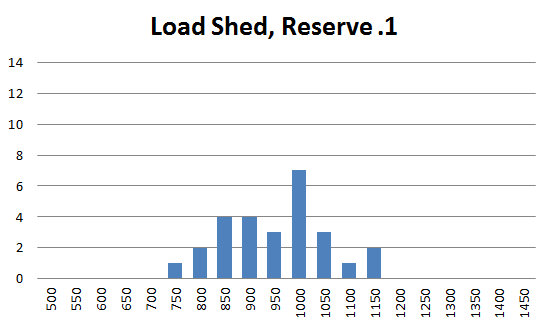
\includegraphics[scale=.75]{reserve1.jpg} \\
     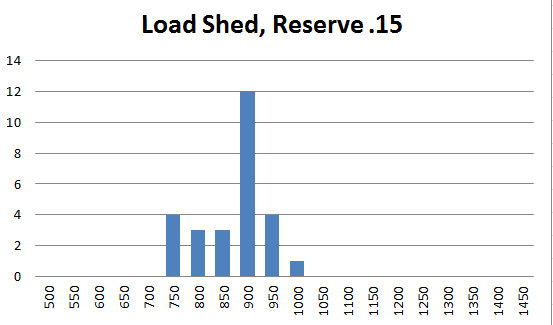
\includegraphics[scale=.75]{reserve15.jpg}
   \end{center}